\documentclass[crop,tikz]{standalone}

\tikzset{>=latex}
\usetikzlibrary{calc}

\begin{document}
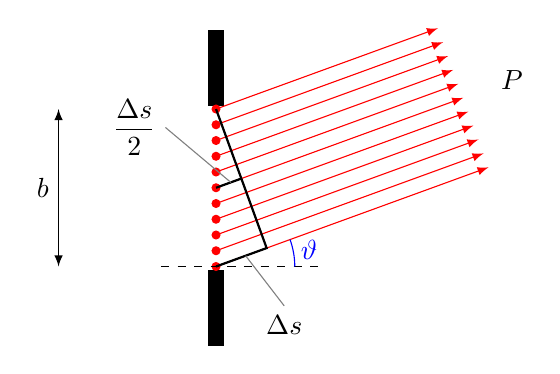
\begin{tikzpicture}
  % slit
  \draw[fill] (-0.1, 1.05) rectangle (0.1, 2.0);
  \draw[fill] (-0.1,-1.05) rectangle (0.1,-2.0);
  % rays
  \foreach \Y in {-1,-0.8,...,1} {%
    \draw[fill,red] (0,\Y) circle (0.05);
    \draw[->,red] (0,\Y) -- +(20:{3+(1-\Y)*sin(20)});
  };
  \node at (20:4) {$P$};
  \draw[dashed] (-0.7,-1) -- (1.3,-1);
  \draw[blue] (0,-1)+(0:1) arc (0:20:1);
  \node[blue] at ($(0,-1)+(10:1.2)$) {$\vartheta$};
  \draw[<->] (-2,-1) -- node[left] {$b$} +(0,2);
  % triangle
  \draw[thick] (0,1) -- +(-70:{2*cos(20)}) -- (0,-1);
  \draw[thick] (0,1)+(-70:{cos(20)}) -- (0,0);
  \draw[gray] (0,-1)+(20:0.4) -- +(-30:1) node[below,black] {$\Delta s$};
  \draw[gray] (0,0)+(20:0.2) -- +(130:1) node[left,black] {$\displaystyle\frac{\Delta s}{2}$};
\end{tikzpicture}
\end{document}
